\documentclass[12pt,a4paper]{article}
\usepackage{graphicx}
\usepackage{array}
\graphicspath{ {/} }
\title{Cross-Plaform Application Development using React Native}
\author{ Sanket Sabale }
%\date


\begin{document}


\maketitle
\newpage
\tableofcontents
\newpage




\section*{Abstract}

 React Native is an Open-Source UI software Framework created by Meta Platforms, in 2015. It is Used to Develop Applications for Android and IOS By enabling developers to use React Framework along with native platform capabilities. It is also being used to develop virtual reality applications at Oculus. The Working Principle of React native are virtually identical to React except that React Native does not manipulate the DOM via the Virtual DOM. It runs in a background process (which  interprets the JavaScript written by the developers ) directly on the end-device and communicates with the native platform via serialized data over an asynchronous and batched bridge. React Components wrap existing native code and interact with native API’s via React’s declarative UI paradigm and JavaScript. While React native styling has a similar sytax to css it does not use HTML or CSS. Instead, messages from the JavaScript thread are used to manipulate native views. React Native also allows developers to write native code in languages such as Java or kotlin for Android, objective-c or swift for ios, and C++/WinRT or  for Windows 10, Which makes it even more flexible Microsoft builds and maintain React Native for windows and React native for macOs.

\addcontentsline{toc}{section}{Abstract}

\newpage

\section*{Motivation}

Today React Native is Accepted By Many Different Companies and They are Hiring React Native Developers . \\
\begin{figure}[h]
    \centering
    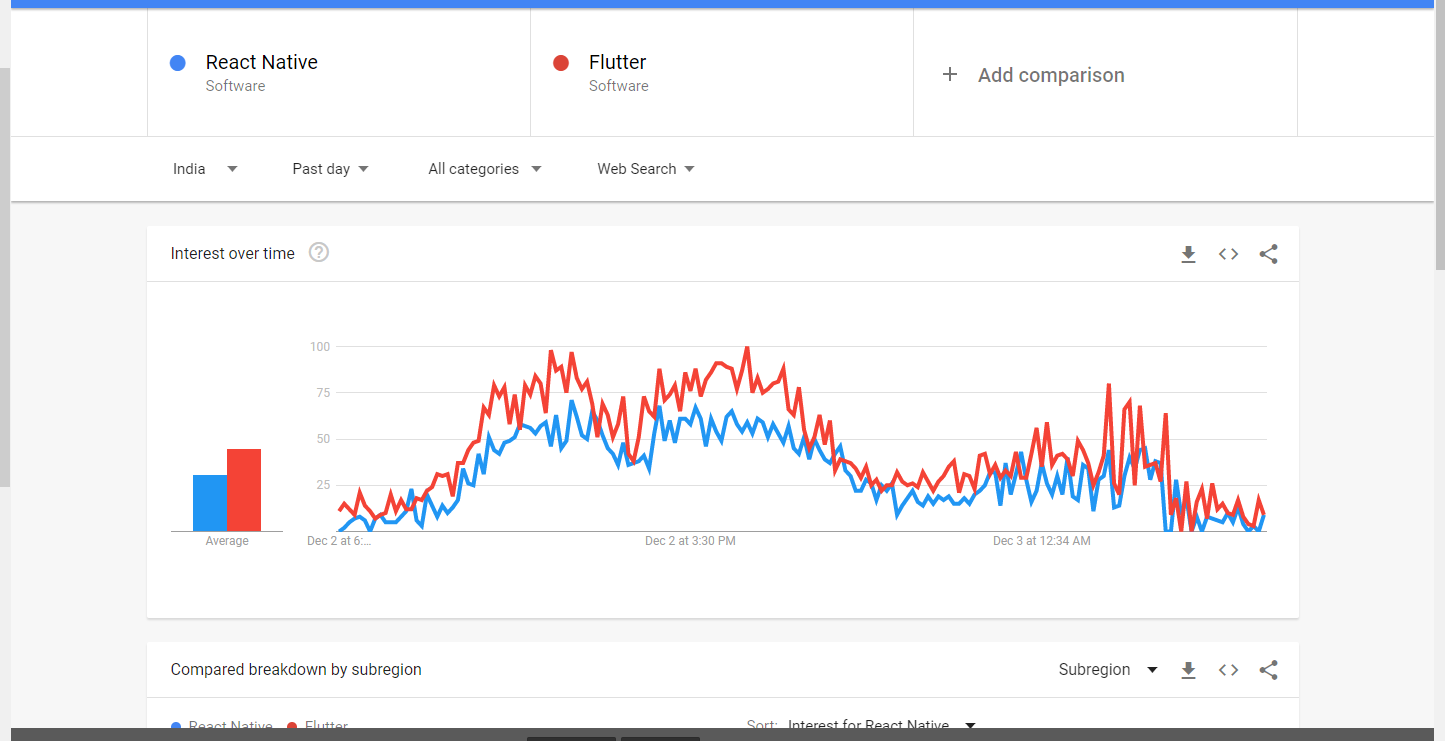
\includegraphics[width=0.55\textwidth]{react_trends}
\end{figure}
\\
 \qquad Also React Native is doing a greate job to beat the other alternatives.We all know that Android users are huge as compare to another platforms and thats why there are millions of apps are downloaded every day so demand of an android developers are really big so if you are wanted to become an android developer you need to pick a perticular android technology but if you have knowledge of web development like JS,HTML,CSS and ReactJS You can Continue with it and you can master these development with React Native. It is a Greate Platform who can give you authority to write code once and make or convert it in IOS and Android App so you don't need to write code for android and ios differently so the big problem are going to be fixed up here. React Native is really gone to easy who are in web development you can connect any backend framework to the android app which is build with react native also there are few other tech as well where you can connect backend but in react native it is easy to connect.

\addcontentsline{toc}{section}{Motivation}
\newpage

\section*{Literature Survey}
\addcontentsline{toc}{section}{Literature Survey}
\subsection*{React Native Based Mobile App for Online Experimentation}
\addcontentsline{toc}{subsection}{React Native Based Mobile App for Online Experimentation}
\begin{tabular}{ |c | m{2.5cm} | m{2cm}| c | m{2cm} | m{2cm} | c | }

  \hline
  sr.no & Title of Page & Author & Published Year & Finding & Future Scope  \\ 
  \hline
  1 & React Native Based Mobile App for Online Experimentation & Xingwei Zhou etal. &  2020 & IEEE Xplore & Helps Student To  get Practicle Exprerince Through 3D \\
\hline 
  
\end{tabular}
\\
\\
\\
In These Article We Found That Author is Telling us That How a Laboratory can be an online tool for everyones use by react native so basically The Concept is there are so many collages which don't have 
practical lab so we can create an app for those student so that he can practice on 3D images and Touchable Effects its looks similar to real practice in it so we can solve a problem of Practical labs in all collages but there some things That i like to update is that we can improve thos UI for students and every single branch needs there own space for practice it also we can include some of test exams so that teacher can see knowledge of student or What he gain? so far.
\\
\\
\newpage
\subsection*{React Native Supplements}
\addcontentsline{toc}{subsection}{React Native Supplements}
\begin{tabular}{ |c | m{2.5cm} | m{2cm}| c | m{2cm} | m{2cm} | c | }

 \hline
  sr.no & Title of Page & Author & Published Year & Finding & Future Scope  \\ 
  \hline
  2 & React Native Supplements & Paul etal. &  2019 & Springer & Guide For Developers \\
\hline 
  
\end{tabular}
\\
\\
\\
These Article is written for help to understand the backend code of React Native. In these Reflux Patterns are explained in very different and Easier manar so that if react native developers whants to implement somethings they get help from these pattern not only these article also tells about Redux the big state management tools to manage states Many of the industries are actually working on it.
So These Articles also tells about how to use redux? How the you can debugg your apps in android phone using deugging mode. But we can implement some libraries for easy development and we can import statements to import more packets. There are lots of things are covered in these article and its helpfull when wants to understand React native deep concepts but for now we have lot more libraries that comes with pre-builted code that help us to us functionality directly on our App.


\newpage
\subsection*{Mobile Development in Swift, Java and React Native}
\addcontentsline{toc}{subsection}{Mobile Development in Swift, Java and React Native}
\begin{tabular}{ |c | m{2.5cm} | m{2cm}| c | m{2cm} | m{2cm} | c | }

  \hline
  sr.no & Title of Page & Author & Published Year & Finding & Future Scope  \\ 
  \hline
  3 &  Mobile Development in Swift, Java and React Native & Hugo Brito etal. &  2019 & IEEE Xplore & Comparing Technologies \\
\hline 
  
\end{tabular}
\\
\\
\\
We know that there are so many technologies are present in the market for creating Android and IOS apps but which is best and how we can found it? The perticular question is solved in these article. while we are creating a Native App we are using Java For android and swift for IOS and to create a both platform application we are using React Native. In native application we found that the performnce of it is really good as compaire to react native but to use more and different library  we need to write to much heavy code and these may be possible that library not presented so we need to manage lots more things to get that functionality done in native apps so that React native solve our problem my suggestion will be like go for react native its saves your time for writing the code which already present and we can compair with these react native with some more cross-plaforms like flutter  and Ionic.

\newpage
\subsection*{JavaScript in Mobile Applications: React native vs Ionic vs NativeScript vs Native Development}
\addcontentsline{toc}{subsection}{JavaScript in Mobile Applications: React native vs Ionic vs NativeScript vs Native Development}

\begin{tabular}{ |c | m{2.5cm} | m{2cm}| c | m{2cm} | m{2cm} | c | }

  \hline
  sr.no & Title of Page & Author & Published Year & Finding & Future Scope  \\ 
  \hline
 4 &  JavaScript in Mobile Applications: React native vs Ionic vs NativeScript vs Native Development & Anabela Gomes etal. &  2018 & IEEE Xplore & Comparing Technologies \\
\hline 
  
\end{tabular}
\\
\\
\\
These Article Also Compare React native with other technologies but Its Compare with cross-platforms mean the other platforms also work as like a react native and by these comparison we are getting best idea to which tech is used for what kind of projects? and you can pick a grate platform. In lot more cases the tech you pick is not suitable for that perticular project may be the other tech performs better then your's in that case you need to use another tech for it that explaination is inside these article but my opinion will be to improve or add other platforms to like flutter and again compare with it because flutter is also a greate tool it usages a dart programming language and its more over an object oriented programming language  so the code you are writing is in classes and object its not a functional base thats the big disadvantage of flutter but its also quite popular in the market now.

\newpage
\subsection*{Exploration of React Native Framework in designing a Rule-Based Application for healthy lifestyle education}
\addcontentsline{toc}{subsection}{Exploration of React Native Framework in designing a Rule-Based Application for healthy lifestyle education}

\begin{tabular}{ |c | m{2.5cm} | m{2cm}| c | m{2cm} | m{2cm} | c | }

  \hline
  sr.no & Title of Page & Author & Published Year & Finding & Future Scope  \\ 
  \hline
 5 &  Exploration of React Native Framework in designing a Rule-Based Application for healthy lifestyle education & Anik Hanifatul Azizah etal. &  2021 & IEEE Xplore & Lifestyle and Education \\
\hline 
  
\end{tabular}
\\
\\
\\
As  we know in these world is Going to faster tech world and now healthy lifestyles is going to be little bit hard for us to find so that these article tells us how we can live a helthy life styles using React Native Rule-Based Application these application comes with some basic rools so that excising and drinking and some more task can be done throught out the notification functionality and some more functionality so that lifestyle becomes technical healthy. But After read these article i think that there are more things we can improve on to it like exerise videos and basic audio file for stress free brain and some more things but all the way these is greate things to work on it and for the healthy lifestyle these ideal is greate to work on it.





\end{document}